\section{camera  Class Reference}
\label{classcamera}\index{camera@{camera}}
Hold location and orientation of the viewer. 


{\tt \#include $<$camera.hpp$>$}

Inheritance diagram for camera::\begin{figure}[H]
\begin{center}
\leavevmode
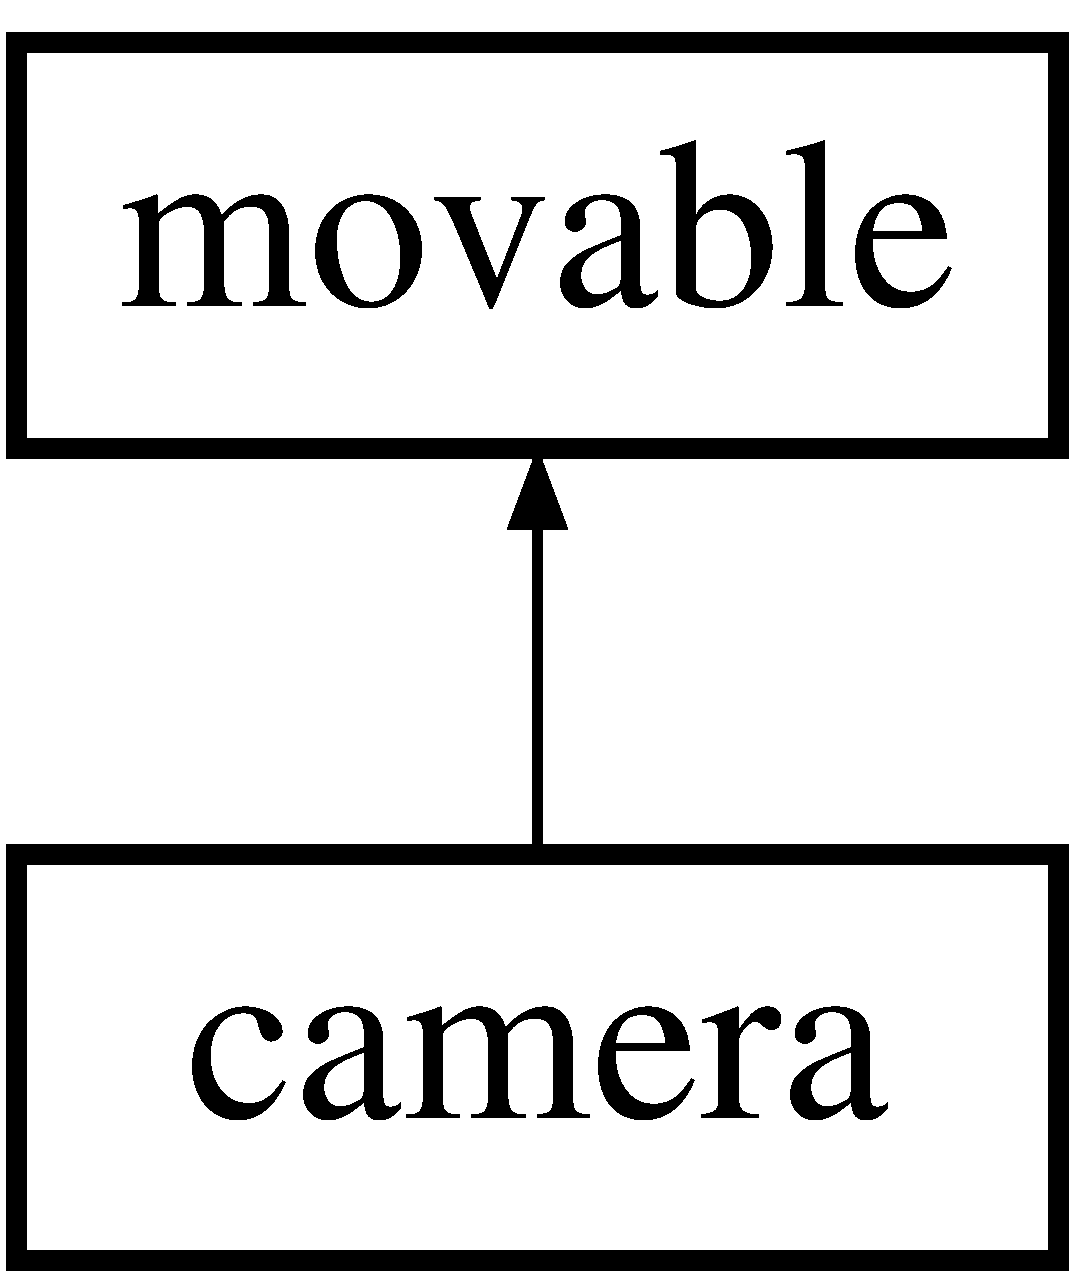
\includegraphics[height=2cm]{classcamera}
\end{center}
\end{figure}
\subsection*{Public Methods}
\begin{CompactItemize}
\item 
\index{camera@{camera}!camera@{camera}}\index{camera@{camera}!camera@{camera}}
{\bf camera} ()\label{classcamera_a0}

\item 
\index{camera@{camera}!camera@{camera}}\index{camera@{camera}!camera@{camera}}
{\bf camera} (char $\ast$name)\label{classcamera_a1}

\item 
\index{~camera@{$\sim$camera}!camera@{camera}}\index{camera@{camera}!~camera@{$\sim$camera}}
{\bf $\sim$camera} ()\label{classcamera_a2}

\item 
\index{init@{init}!camera@{camera}}\index{camera@{camera}!init@{init}}
void {\bf init} ()\label{classcamera_a3}

\item 
\index{draw@{draw}!camera@{camera}}\index{camera@{camera}!draw@{draw}}
void {\bf draw} ()\label{classcamera_a4}

\item 
\index{update@{update}!camera@{camera}}\index{camera@{camera}!update@{update}}
void {\bf update} ()\label{classcamera_a5}

\item 
\index{look@{look}!camera@{camera}}\index{camera@{camera}!look@{look}}
void {\bf look} (void)\label{classcamera_a6}

\end{CompactItemize}
\subsection*{Public Attributes}
\begin{CompactItemize}
\item 
\index{radius@{radius}!camera@{camera}}\index{camera@{camera}!radius@{radius}}
float {\bf radius}\label{classcamera_m0}

\item 
\index{delay@{delay}!camera@{camera}}\index{camera@{camera}!delay@{delay}}
{\bf matrix16f} {\bf delay} [20]\label{classcamera_m1}

\begin{CompactList}\small\item\em the most recent center locations, the camera follows the last.\item\end{CompactList}\item 
\index{other@{other}!camera@{camera}}\index{camera@{camera}!other@{other}}
{\bf matrix16f} {\bf other}\label{classcamera_m2}

\begin{CompactList}\small\item\em extra matrix needed for follow mode.\item\end{CompactList}\item 
\index{center@{center}!camera@{camera}}\index{camera@{camera}!center@{center}}
{\bf matrix16f} $\ast$ {\bf center}\label{classcamera_m3}

\begin{CompactList}\small\item\em Location for camera to spin around.\item\end{CompactList}\item 
\index{mode@{mode}!camera@{camera}}\index{camera@{camera}!mode@{mode}}
int {\bf mode}\label{classcamera_m4}

\end{CompactItemize}


\subsection{Detailed Description}
Hold location and orientation of the viewer.

Also some experimental modes of movement  like following a given object, and following that objects every rotation, same with a delay, or just tracking the object without rotating with it. 



The documentation for this class was generated from the following files:\begin{CompactItemize}
\item 
{\bf camera.hpp}\item 
camera.cpp\end{CompactItemize}
